\section{Structure de la plateforme}

Une fois les outils de collaboration choisis, le choix des technologies de programmation ainsi que la structure du projet allaient devoir être explicités. Pour nos besoins, nous avons tout de suite su quel modèle architectural nous allions choisir: \textbf{une API RESTful monolithique}.\\

\begin{figure}[th]
\centering
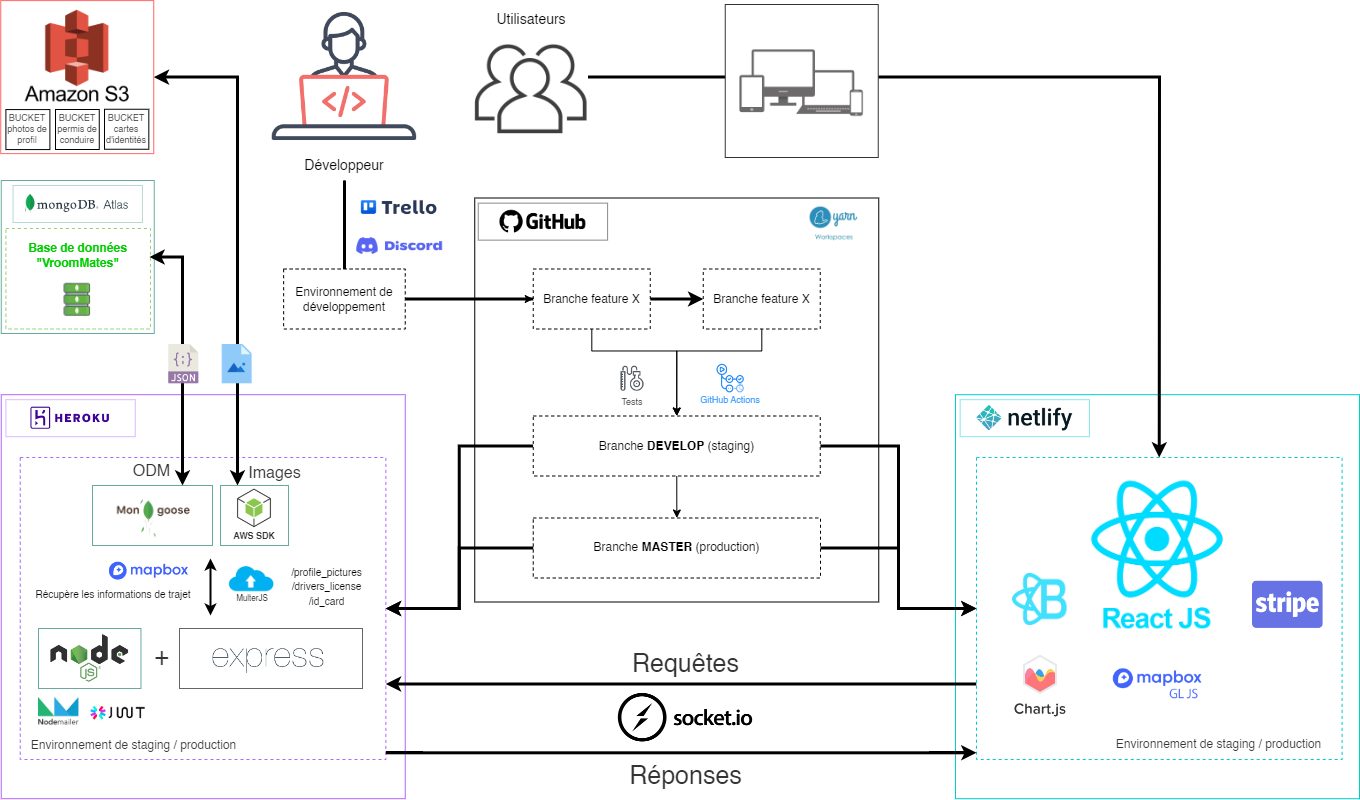
\includegraphics[width=\linewidth]{medias/stack-structure.png}
\decoRule
\caption{Structure de la stack technique (voir en grand: \ref{Stack technique complète du site})}
\end{figure}

\subsection{Une architecture monolithique}

Une architecture monolithique est formée d'un seul bloc regroupant l'intégralité de nos services: avec l'interface utilisateur, la logique métier, l'interface de données, ainsi que la base de données.

Cette architecture nous a permis de centraliser notre code dans un seul et même repository (dépôt) → Il s'agit de l'architecture mono-repo\parencite{Ref1}. 

Nous utiliserons \textbf{Yarn Workspace} afin de profiter des avantages de ce type d'architecture (un seul fichier lockfile, toutes les dépendances installés au même endroit, une gestion des tests plus simple).

\textbf{Toute la codebase sera donc accessible publiquement via ce lien GitHub: \href{https://github.com/agerard57/VroomMates}{https://github.com/agerard57/VroomMates}.}


\subsection{Structure de la base de données}

Nous avons, pour cette partie, beaucoup effectué de tests et de recherche, non-seulement pour trouver quel outil utiliser (MongoDB, DynamoDB, ElasticSearch, mySQL, etc…), mais déjà pour savoir quel type de schéma la table allait avoir.
Pour cela, nous devions déjà répertorier quelles données allaient être stockées;
Hormis les éléments stockables dans une base de données relationnelle "classique" (comme par exemple les données sur un utilisateur), nous avions des données plus spécifiques à notre projet à entreposer: il fallait trouver un moyen de stocker des positions géographiques (un trajet = point A → point B). C'est pour cela que nous nous sommes tournés vers \textbf{les bases de données document}.

Étant un système de documents non relationnel, nous pouvons imbriquer des listes et des objets, ce qui s'avère pratique pour des coordonnées. 
Nous allons donc utiliser de façon plus précise \textbf{MongoDB}: nous pouvons ainsi utiliser leur possibilité de stockage d'objets \textbf{GeoJSON}\parencite[]{Ref2}.\\ Notre base de donnée sera déployée dans le cloud et uniquement accessible par l'api grâce à la mise en place du service \textbf{MongoDB Atlas}.\\

Voir le modèle de la base de données: \ref{Modèle non-relationnel de la base de données}\\

En plus de MongoDB, un système de stockage d'objets allait devoir être mis en place afin de garder des images comme les photos de profil ainsi que les permis de conduire). Nous avons sélectionné \textbf{Amazon S3}, l'un des membres du groupe étant déjà familier avec le service.


\subsection{Structure coté client}

Côté client, après avoir fait la recherche de l'existant sur le point technique (voir \ref{Stack technique}), et, avec l'expérience pré-acquise, nous allons nous diriger vers \textbf{ReactJS, en TypeScript}. Une grande rigueur sera attendue au niveau de la qualité du code, puisque ce dernier sera testé par des outils comme ESlint, prettier, prettier-sort-imports, etc…. Nous allons nous aider de React-Bootstrap au niveau de la réalisation de la responsiveness.
Sur ce thème, nous allons d'ailleurs adopter une approche "\textbf{mobile-first}", vu la nature de la plateforme.
En ce qui concerne les api externes, nous seront aidés de \textbf{Stripe} (pour les paiements) et \textbf{mapbox} (pour les cartes). Le tout sera automatiquement déployé sur Netlify grâce à notre système de CI/CD. 

L'URL du site étant par défaut accessible uniquement par un sous-domaine netlify (\href{https://tourmaline-cascaron-c8cbd7.netlify.app}{https://tourmaline-cascaron-c8cbd7.netlify.app}), nous avons décidé de rediriger le client vers un TLD personnel, question de simplicité et d'esthétisme. Le site sera donc accessible au sous-domaine \textbf{\href{https://www.vroommates.agerard.dev}{https://www.vroommates.agerard.dev}}. Cela nous permettra d'avoir une URL plus présentable sans pour autant dépenser pour un nouveau domaine. Le déploiement du site n'étant pas demandé initialement, cela nous permettra de pratiquer certains aspects de création de site que nous n'aurions pas pu faire si nous étions restés uniquement en local (par exemple, de la CI/CD ou de la SEO)…

\subsection{Structure coté API}

Afin de se conformer aux choix de langages du client, nous avons décidé d'utiliser \textbf{NodeJS + Express.js, en JavaScript}.
Dans cette partie du projet, plusieurs outils ont été pensés à des fins bien précises:
\begin{itemize}
\item Pour les fonctionnalités de chat, étant donné la création d'un système de messagerie instantanée, nous avons opté pour \textbf{socket.io}
\item Pour la protection des routes et pour l'authentification, \textbf{JWT} nous permettra d'utiliser leurs jetons.
\item Pour relier la base de données MongoDB et l'API, nous utiliserons un ODM, précisément \textbf{Mongoose}
\item L'API de \textbf{mapbox} nous servira à récupérer des informations sur le trajet (principalement convertir des coordonnées en nom de rue/ville)
\item Afin de valider l'adresse Email de l'utilisateur, nous allons utiliser le module \textbf{NodeMailer} qui va envoyer des codes de confirmation par ce même biais.
\item Comme précisé plus tôt, étant donné que nous avons besoin de stocker des images, nous ne voulions pas simplement les stocker sur le serveur avec \textbf{MulterJS}. Nous nous en servons alors juste pour stocker une image le temps de l'envoyer dans son bucket S3 respectif avec \textbf{AWS SDK}
\end{itemize}

Nous avons donc eu, tout comme le client, l'intention de déployer l'API sur un serveur. Nous utiliserons les service d'\textbf{Heroku}. Ce dernier est disponible à l'adresse suivante: \textbf{\href{https://vroommates-agerard57.herokuapp.com/}{https://vroommates-agerard57.herokuapp.com/}}\\

\textit{Notons que nous n'avons pas besoin de changer le nom de domaine / sous-domaine car ce dernier ne sera utilisé uniquement que par le client, et non pas directement l'utilisateur.}

\subsection{CI/CD}

Notre plateforme aura aussi la particularité de proposer un système avancé de CI/CD.
Pour commencer, notre repository utilisera les fonctionnalités de github actions. 

Voici le fonctionnement d'un déploiement:

\begin{itemize}
\item Avant chaque pull request vers la branche "develop", nous metterons en place des workflows qui vérifieront la bonne mise en forme du code (eslint, prettier, sort imports) ainsi que de la documentation (markdownlint);
\item Ensuite, un second set de workflows feront des tests unitaires, des tests d'intégration, des tests end-to-end et/ou des tests d'acceptation.
Nous utiliserons Jest couplé avec Pupeteer pour ces tests;
\item Une phase de code review entre nos membres va dès lors se faire;
\item Enfin, après notre validation, lors du merge (fusion) vers la branche "develop", un dernier set de workflows va respectivement déployer le "front-end" et le "back-end" à Netlify et Heroku. Bien évidemment, ces workflows ne vont se déclencher qu'à la réussite des précédents tests. On vérifie donc une dernière fois que toutes les features sont fonctionnelles en staging, puis on passe le tout en production. 
\end{itemize}
